\section{Các chương trình test}
\subsection{Chương trình \textit{help}}
Chương trình \textit{help} gọi syscall PrintString để in thông tin về nhóm cũng như giới thiệu vắn tắt về chương trình \textit{ascii} và chương trình \textit{sort}.
\begin{figure}[H]
\begin{center}
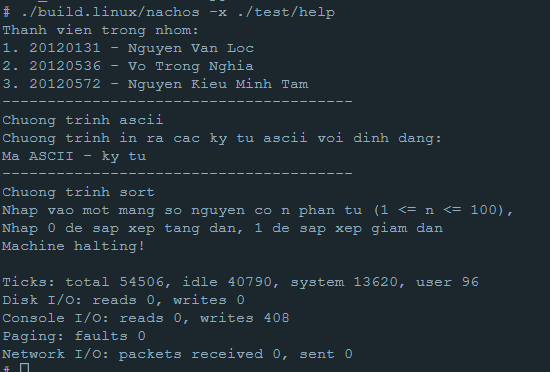
\includegraphics[scale=1]{help}
\end{center}
\caption{Chương trình \textit{help}}
\end{figure}

\subsection{Chương trình \textit{ascii}}
Chương trình \textit{ascii} chủ yếu sử dụng \textit{PrintChar}, \textit{PrintString}, và \textit{PrintNum} để in mã ASCII và ký tự tương ứng.\\
\textbf{Lưu ý:} Chỉ những ký tự in được mới có thể hiện lên màn hình.\\
Hình ảnh chương trình \textit{ascii}:
\begin{figure}[H]
\begin{center}
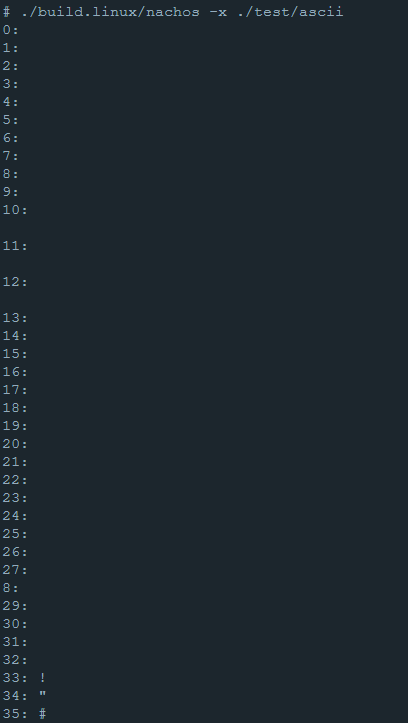
\includegraphics[scale=1]{ascii_1}
\end{center}
\caption{Chương trình \textit{ascii}}
\end{figure}

\begin{figure}[H]
\begin{center}
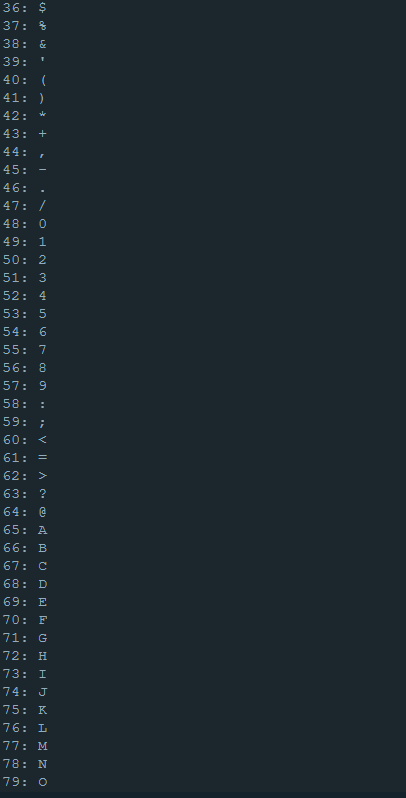
\includegraphics[scale=1]{ascii_2}
\end{center}
\caption{Chương trình \textit{ascii}}
\end{figure}

\begin{figure}[H]
\begin{center}
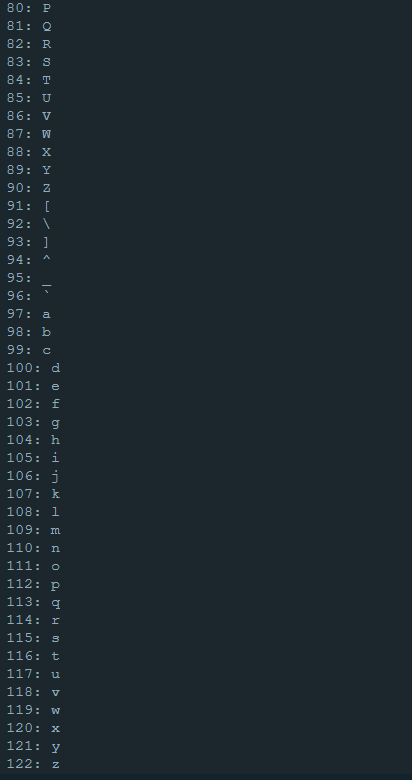
\includegraphics[scale=1]{ascii_3}
\end{center}
\caption{Chương trình \textit{ascii}}
\end{figure}

\begin{figure}[H]
\begin{center}
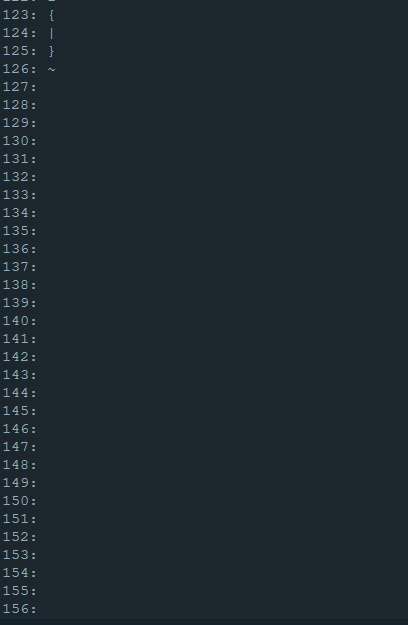
\includegraphics[scale=1]{ascii_4}
\end{center}
\caption{Chương trình \textit{ascii}}
\end{figure}

\subsection{Chương trình \textit{sort}}
Chương trình sắp xếp tối đa 100 số nguyên tăng dần/giảm dần bằng thuật toán bubble sort.\\
Chương trình sử dụng các syscall \textit{ReadNum}, \textit{PrintNum}, \textit{PrintString}.\\
Hình ảnh chương trình \textit{sort}:
\begin{figure}[H]
\begin{center}
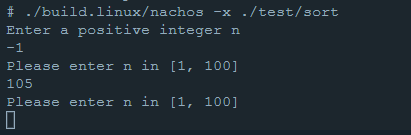
\includegraphics[scale=1]{sort_1}
\end{center}
\caption{Trường hợp $n$ không hợp lệ}
\end{figure}

\begin{figure}[H]
\begin{center}
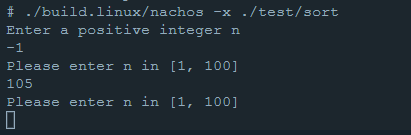
\includegraphics[scale=1]{sort_1}
\end{center}
\caption{Trường hợp sắp xếp tăng dần}
\end{figure}

\begin{figure}[H]
\begin{center}
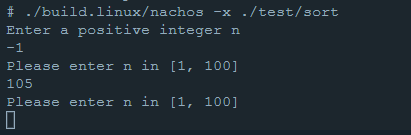
\includegraphics[scale=1]{sort_1}
\end{center}
\caption{Trường hợp sắp xếp giảm dần}
\end{figure}